\documentclass[a4paper,platex,dvipdfmx,twocolumn]{jsarticle} 
\usepackage[left=20mm, right=20mm, top=20mm, bottom=20mm]{geometry}
\usepackage{graphicx}
\usepackage{tabularx, amssymb}
\usepackage{booktabs}
\usepackage{multirow}
\usepackage{afterpage}
\usepackage{titlesec}
\usepackage{cite}
\usepackage{algorithm}
\usepackage{algpseudocode}
\usepackage{amsmath}

\makeatletter
% --- \section の書式を jsarticle シングルカラムと同じ程度に ---
\titleformat{\section}{\reset@font\Large\gtfamily\bfseries}{\thesection}{1em}{}

% --- \subsection の書式を jsarticle シングルカラムと同じ程度に ---
\titleformat{\subsection}{\reset@font\large\gtfamily\bfseries}{\thesubsection}{1em}{}

% \titlespacing*{\section}{0pt}{2.3\baselineskip plus 0.5\baselineskip minus 0.2\baselineskip}{0.9\baselineskip}

% \titlespacing*{\subsection}{0pt}{1.5\baselineskip plus 0.4\baselineskip minus 0.2\baselineskip}{0.5\baselineskip}

% % タイトルと表のための独立したページ用のマクロを定義
% \makeatletter
\def\@maketitle{%
  \begin{center}
    {\LARGE 修 士 論 文 要 旨\par}
    \vspace{6pt}
    {Summary of the Master's Thesis\par}
    \vspace{20pt}
    % 表をタイトルページの一部として組み込む
    \begin{tabular}{|p{25mm}|p{50mm}|p{25mm}|p{50mm}|}
      \hline
      \centering{学 生 番 号} & M243422 & \centering{プ ロ グ ラ ム} & 情報科学プログラム\\
      \centering{\scriptsize{Student ID number}} && \centering{\scriptsize{Program}} & \\
      \hline
      \centering{氏　　　名} & 廣池 友哉 & \centering{主 指 導 教 員} & 古居 彬\\
      \centering{\scriptsize{Name}} && \centering{\scriptsize{Supervisor}} & \\
      \hline
      \centering{論 文 題 目} & \multicolumn{3}{|l|}{不確実性適応型損失関数による頑健な医用画像セグメンテーション}\\
      \centering{\scriptsize{Thesis Title}} & \multicolumn{3}{|l|}{}\\
      \hline
    \end{tabular}
  \end{center}
  \vspace{30pt}  % タイトルと本文の間のスペース
}
% \makeatother

\begin{document}
% タイトルと表を表示
\twocolumn[{\maketitle}]

\section{はじめに}

医用画像セグメンテーションは，診断支援や治療計画において不可欠な技術であり，
正常組織または異常組織の領域を抽出することが求められる．
特に大腸ポリープ\cite{ji2022video}や頭頸部がん放射線治療における危険臓器\cite{maleki2020machine}の検出など，臨床応用が進んでいる．

しかしながら，医用画像セグメンテーションには固有の課題が存在する．特に重要な問題として，クラス不均衡が挙げられる．
医用画像では背景領域が大部分を占め，対象となる病変は相対的に小さい領域しか占めないことが多い．
この状況下では，従来の分類タスクで広く使われているCross-Entropy Loss\cite{long2015fully}は背景領域の学習に偏り，
臨床的に重要な小病変や曖昧な境界部分の正確なセグメンテーションが困難となる．

この課題に対処するため，クラス不均衡に対して頑健なDice Loss\cite{milletari2016v}やその
多くの拡張手法が提案され，CT画像\cite{zhu2019anatomynet, 9109297}や
MRI画像\cite{KATO2024107695}において高い性能が報告されている．
しかし，これらの損失関数は全画像に対して固定的な形状を持つという制約がある．
医用画像は，撮影条件や個体差に加え，病変サイズ・形状の著しいばらつき，組織間のコントラストの違い，
あるいは境界の不明瞭さなどといった大きな多様性を有しており，画像ごとにセグメンテーションの難易度が大きく異なる．
固定的な損失関数を用いると，容易な画像と困難な画像に対して同一の学習信号を与えるため，困難な画像に対する学習が不十分となる可能性がある．
したがって，画像ごとの難易度に応じて損失関数を適応的に調整するアプローチが有望である．
このような適応的学習の実現には，2つの要素が求められる．1つは，難易度の高い画像に対して学習信号を強化できるよう，
損失関数の形状を柔軟に制御する手法である．
もう1つは，各画像がモデルにとってどの程度困難であるかを学習中に評価するための難易度指標である．

本研究では，これら2つの要素を統合した適応的学習フレームワークを提案する．
損失関数の形状制御には，Dice Lossを多項式展開して得られるPolyDice Loss\cite{polydice}を
用いる．PolyDice Lossは画像毎に最適なパラメータを用いて
損失関数の形状を連続的に制御できるため，適応的学習に適している．
難易度の定量化には，Monte Carlo Dropout\cite{pmlr-v48-gal16}（以下，MC Dropout）による
不確実性推定を用いる．
MC Dropoutは，推論時にDropoutを有効にすることで，モデルの認識的不確実性を効率的に推定できる．
この不確実性は，モデルがその画像のセグメンテーションにおいてどの程度の確信を持てないかを反映しており，セグメンテーション難易度の指標として利用可能である．
提案手法では，推定された不確実性指標に基づきPolyDice Lossの形状パラメータを動的に制御し，
困難な画像には急峻な勾配を，容易な画像には緩やかな勾配を与えることで，効率的かつ頑健な学習の実現を目指す．

本研究の主要な貢献は以下の通りである．
\begin{enumerate}
    \item \textbf{不確実性に基づく画像難易度の動的定量化手法の導入：}
    MC Dropoutを用いて推論時の認識的不確実性を推定し，これを画像単位の「学習難易度」として定量化する手法を提案する．
    これにより，医用画像の多様なセグメンテーション難易度を，モデル自身の確信度に基づいて客観的に評価することを可能にする．

    \item \textbf{難易度に応じた損失関数の適応的制御フレームワークの構築：}
    定量化された難易度指標に基づき，PolyDice Lossの形状パラメータを適応的に制御する学習フレームワークを構築した．
    提案法は，学習の進行に伴い変化する難易度に応じて損失関数の勾配を自動調整することで，困難な症例への学習の注力と，容易な症例による勾配支配の抑制を同時に実現する．

    \item \textbf{複数のデータセットを用いた有効性と汎用性の実証：}
    医用画像データセットを用いた比較実験により，提案手法の有効性を検証した．
    実験の結果，従来の形状が固定された損失関数と比較してセグメンテーション精度が向上することを示した．
\end{enumerate}

\section{予備知識}
\subsection{PolyDice Loss}
医用画像セグメンテーションで広く使用されるDice Lossは，クラス不均衡に頑健であるが，全画像に対して固定的な形状を持つという制約がある．
本研究では，Dice Lossを多項式展開により拡張したPolyDice Loss\cite{polydice}，特にその実用的な形式であるPolyDice-1 Lossを採用する．
PolyDice-1 Lossは，単一のパラメータ$\epsilon$で損失関数の形状を制御でき，画像の難易度に応じて勾配の急峻さを調整することが可能となる．

\subsubsection{Dice Lossの定義}
画像サイズを $H \times W$とし，ピクセル位置を $(i, j)$ で表す
$\left(i \in \{1, ..., H\}, j \in \{1, ..., W\}\right)$．
セグメンテーションタスクにおいて，モデルの予測確率マップを$\hat{\mathbf{Y}} = \{\hat{y}_{i,j}\}_{i,j} \in \mathbb R ^ {H \times W}$，
その画像に対する正解マスクを$\mathbf{Y} = \{{y}_{i,j}\}_{i,j} \in \mathbb R ^ {H \times W}$とすると，Dice Lossは次式で定義される．

\begin{equation}
    \mathcal{L}_{\text{Dice}}(\hat{\mathbf{Y}}, \mathbf{Y}) = 1 - \frac{2 \sum_{j=1}^{W} \sum_{i=1}^{H} \hat{y}_{i, j} y_{i, j}}{\sum_{j=1}^{W} \sum_{i=1}^{H}(\hat{y_{i, j}} ^ 2 + y_{i, j} ^ 2)}
\end{equation}

\subsubsection{幾何学的解釈と多項式展開}

予測確率マップ$\hat{\mathbf{Y}}$と正解マスク$\mathbf{Y}$をそれぞれ長さ$HW$のベクトル$\hat{\mathbf{y}}, \mathbf{y}$
として平坦化すると，Dice Lossは以下のように分解できる．

\begin{equation}
    \mathcal{L}_{\text{Dice}} = 1 - s \cos \theta
\end{equation}
ここで，$s = \frac{2 \langle \hat{\mathbf{y}}, {\mathbf{y}} \rangle}{\Vert \hat{\mathbf{y}} \Vert ^ 2 + \Vert {\mathbf{y}} \Vert ^ 2}$はスケール成分，
$\theta = \arccos{\frac{\langle \hat{\mathbf{y}}, {\mathbf{y}}\rangle}{\Vert \hat{\mathbf{y}} \Vert \Vert {\mathbf{y}}\Vert}}$は2つの
ベクトル間の角度を表す．この分解により，Dice Lossはスケール成分$s$と$\cos \theta$の積として理解できる．

方向成分$\cos \theta$に対してTaylor展開を適用することで，PolyDice Lossの多項式表現を導出する．
学習が進むにつれて予測$\hat{\mathbf{y}}$は正解$\mathbf{y}$に近づくため，両ベクトルのなす角$\theta$は$0$に近づく．
この性質を利用し，$\cos{\theta}$を$\theta = 0$まわりでテイラー展開すると以下のように近似できる．
\begin{equation}
    \cos{\theta} = 1 - \frac{\theta ^ 2}{2!} + \frac{\theta ^ 4}{4!} - \cdots
\end{equation}
これをDice Lossに代入し，整理するとPolyDiceの一般形が得られる：

\begin{align}
    \mathcal{L}_{\text{PolyDice}} &= 1 - s\left(1 - \frac{\theta ^ 2}{2!} + \frac{\theta ^ 4}{4!} - \cdots\right) \\
    &= (1 - s) + s \sum_{k = 1}^{\infty} \alpha_k \theta ^ {2k}
\end{align}
ここで， $\alpha_k=\frac{(-1)^{k-1}}{(2k)!}$は各Taylor項の符号係数である．

\subsubsection{PolyDice-1 Loss}

PolyLoss\cite{leng2022polyloss}は分類タスクにおいてCross-Entropy Lossを多項式展開し，
第1項のみを調整可能とすることで実用的な性能向上を達成した．PolyDice Loss\cite{polydice}はこのアプローチをDice Lossに適用したものであり，
本研究では第1項のみを調整する PolyDice-1 Loss を採用する．
\begin{equation}
    \mathcal{L}_{\text{PolyDice-1}} = (1 - s) + s \left(\frac{1}{2} + \epsilon\right) \theta^2
\end{equation}
ここで，$\epsilon \in \mathbb{R}$は損失関数の形状を制御するハイパーパラメータである．
図\ref{polydice}に，$\epsilon$に応じたPolyDice-1 Lossの形状変化を示す．
$\epsilon > 0$では予測誤差に対するペナルティが強化され，$\epsilon < 0$では緩和される．
この柔軟な形状制御が可能な特性は，本研究の適応的学習フレームワークにおいて重要な役割を果たす．
後述する提案手法では，この$\epsilon$を動的に調整することで，個々の画像の難易度に応じた勾配制御を実現し，学習戦略をサンプル単位で最適化することを可能にしている．

\begin{figure}
    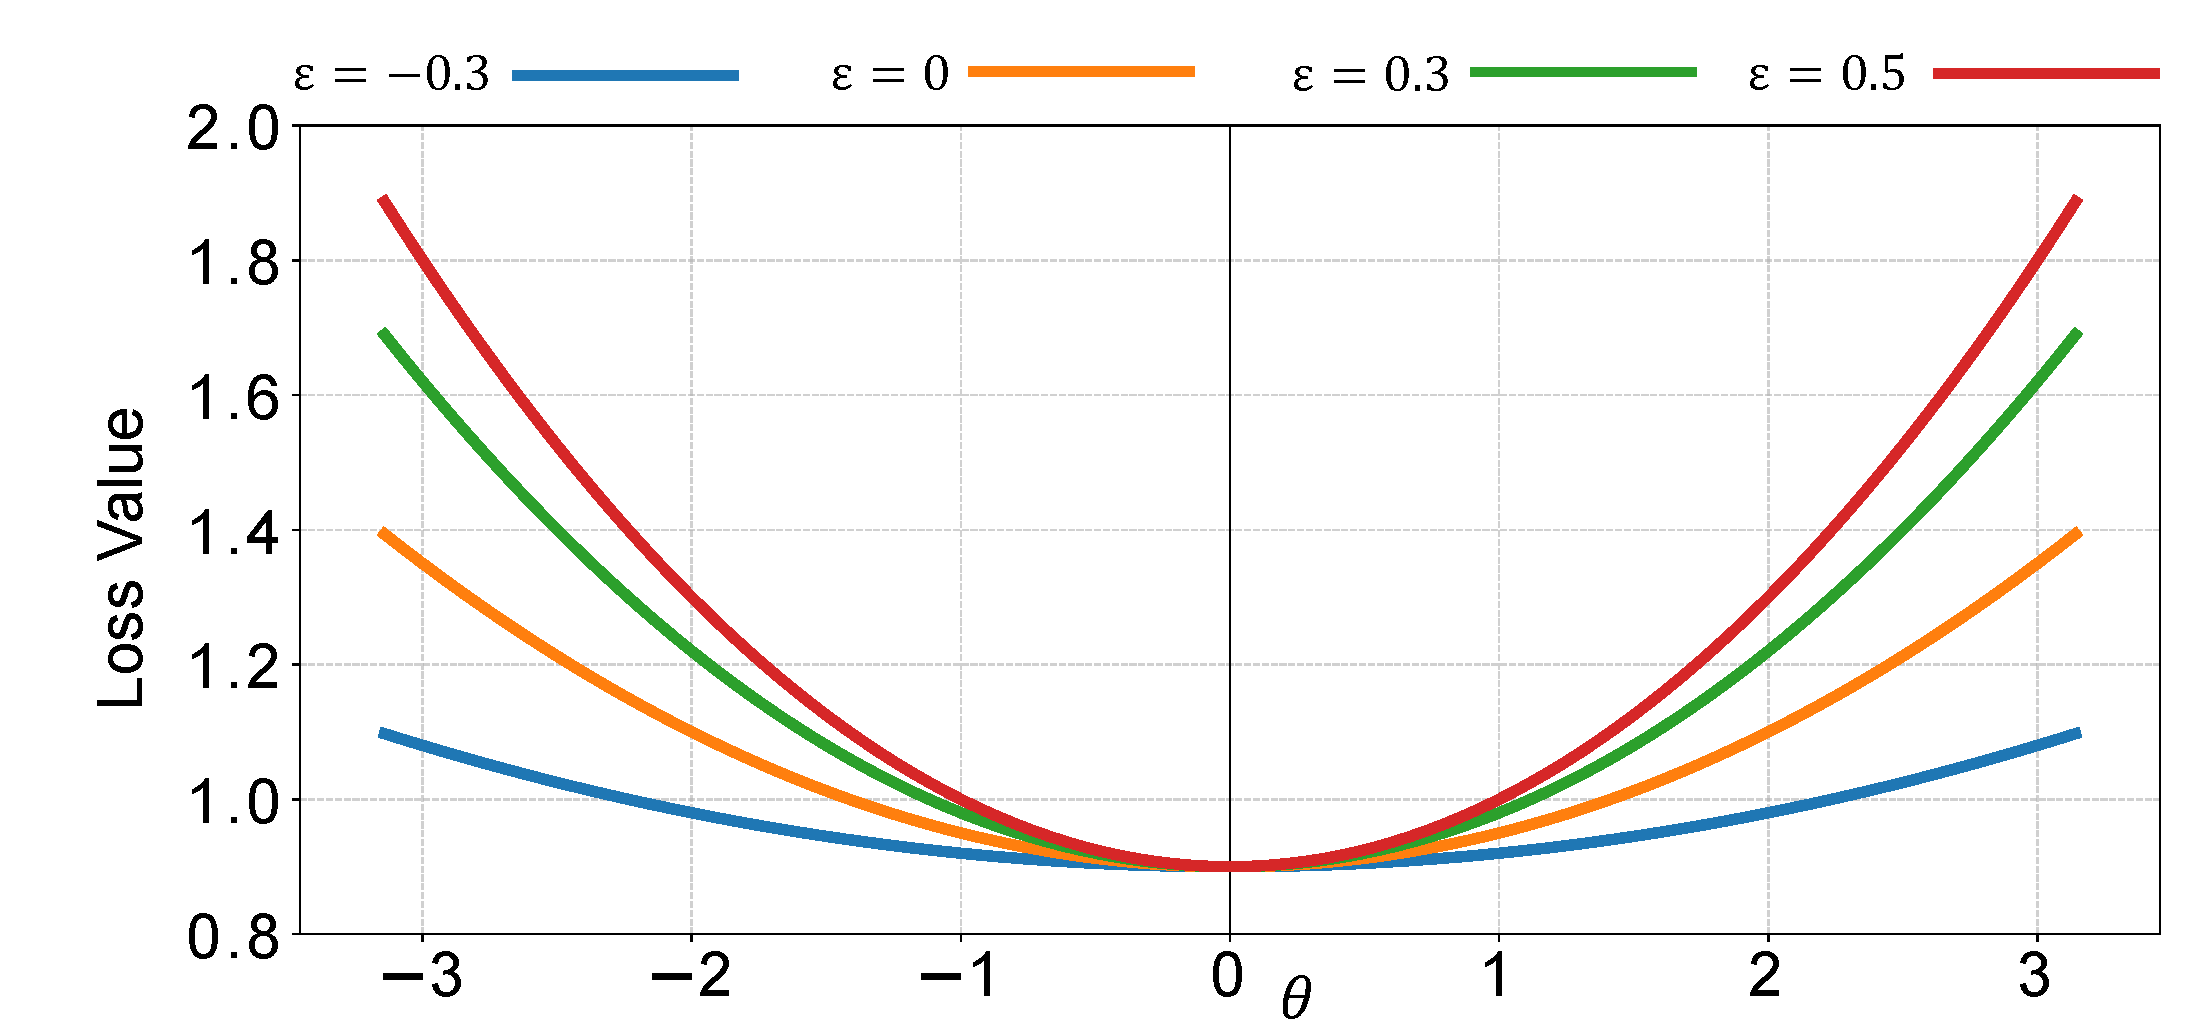
\includegraphics[width=\columnwidth]{figure/loss.pdf}
    \caption{Plot of PolyDice-1 Loss ($s = 0.1$)}
    \label{polydice}
\end{figure}

\subsection{MC Dropout}

\subsubsection{認識的不確実性と偶然的不確実性}

深層学習モデルの予測に伴う不確実性は，その発生源に基づいて偶然的不確実性と認識的不確実性に大別される\cite{smith2018understanding}．

偶然的不確実性（Aleatoric Uncertainty）は，撮像装置に起因するノイズや低解像度，
あるいは組織境界の物理的な曖昧さなど，データそのものに内在する情報不足に起因する．
この不確実性はデータの本質的な統計的性質であるため，同一ドメインの訓練データを追加しても解消されない特性を持つ．

認識的不確実性（Epistemic Uncertainty）は，モデルが未学習のパターンや，
訓練データの不足による知識の欠如に起因する．
これは適切な学習データを追加し、モデルが対象の分布をより詳細に記述することで低減が可能である．
認識的不確実性が高い画像は，モデルが安定した特徴表現を獲得できておらず，予測が不安定な状態にあることを示す．
本研究では，この認識的不確実性を画像のセグメンテーション難易度を反映する指標として活用する．

\subsubsection{MC Dropout の原理と応用}

Dropoutは，ニューラルネットワークの過学習を防ぐ正則化手法として提案された\cite{JMLR:v15:srivastava14a}．
訓練時に各層のニューロンを確率$p$でランダムに不活性化することで，
モデルの汎化性能を向上させる．通常，推論時にはDropoutは無効化され，全ニューロンが活性化された状態で決定論的な予測が行われる．

MC Dropout\cite{pmlr-v48-gal16}は，学習時のみだけでなく，推論時にもDropoutを有効にすることで，モデルの認識的不確実性を推定する手法である．
Dropoutを有効にするした状態で推論を行うと，各推論において異なるニューロンが不活性化されるため，
実質的に異なる部分ネットワークによる予測が得られる．
同一入力に対してこの確率的推論を複数回実行することで，予測の分布を取得できる．

Gal and Ghahramani\cite{pmlr-v48-gal16}は，Dropout を適用したニューラルネットワークの学習が，
ベイズ推論における近似と数学的に等価であることを示した．この理論的枠組みにより，MC Dropout で得られる
予測分布は，モデルパラメータの事後分布に基づく予測不確実性，すなわち認識的不確実性の近似として解釈できる．

提案法では，MC Dropoutによる推定される認識的不確実性を，
画像のセグメンテーション難易度を反映する指標として活用し，損失関数の適応的制御に利用する．



\section{提案法}

\subsection{概要}

訓練データセットを $\mathcal{D} = \{(\mathbf{X}_n, \mathbf{Y}_n)\}_{n=1}^{N}$ とする．
ここで，$N$ は訓練画像の総数，$\mathbf{X}_n \in \mathbb{R}^{H \times W \times C}$ は $n$ 番目の入力画像（$C$はチャンネル数），
$\mathbf{Y}_n = \{y_{n,i,j}\}_{i,j} \in \mathbb{R}^{H \times W}$ は対応する正解マスクである．
MC Dropout による不確実性推定では，各画像に対して $T$ 回の確率的推論を行う．
$t$ 回目の推論（$t \in \{1, \ldots, T\}$）における予測確率マップを $\hat{\mathbf{Y}}_n^{(t)} = \{\hat{y}_{n,i,j}^{(t)}\}_{i,j}$ と表記する．

図\ref{method} に提案手法の概要を示す．
本手法の設計は，主に以下の2つの観点に基づいている．
第一に，学習サンプルに対する難易度評価を，学習プロセスの中で動的に更新する点である．
画像の難易度は絶対的なものではなく，モデルの学習進捗によって変化する相対的なものであるため，
現在のモデルの状態に基づいて難易度を逐次再評価することで，
その時点でのモデルにとって確信を持てない画像に学習を集中できる．
第二に，難易度の定量化指標として，認識的不確実性が適している点である．
認識的不確実性は「モデルの知識不足」に起因するため，モデルが未学習のパターンや判断に迷っている領域を直接的に反映するため，
ノイズに影響されることなく，学習によって改善可能な「モデルにとってどれくらい確信を持てないか」を適切に定量化することが可能となる．

提案法では，学習中各画像に対して $\tau$ エポックごとに MC Dropout を用いて画像毎に複数枚推論を行い，予測のばらつきから不確実性を定量化する．
この不確実性情報は，モデルがその画像のセグメンテーションにおいてどの程度の確信を持てないかを反映する．
その後，この不確実性情報を画像単位に集約し，PolyDice Loss の形状を動的に制御することで，難しい画像には急峻な勾配を，簡単な画像には緩やかな勾配を与える．
更新された $\epsilon$ を次の $\tau$ エポック間の学習に適用することで，学習の進行度に応じて最適化の重み付けを動的に変化させる適応的学習を実現する．

\begin{figure}
    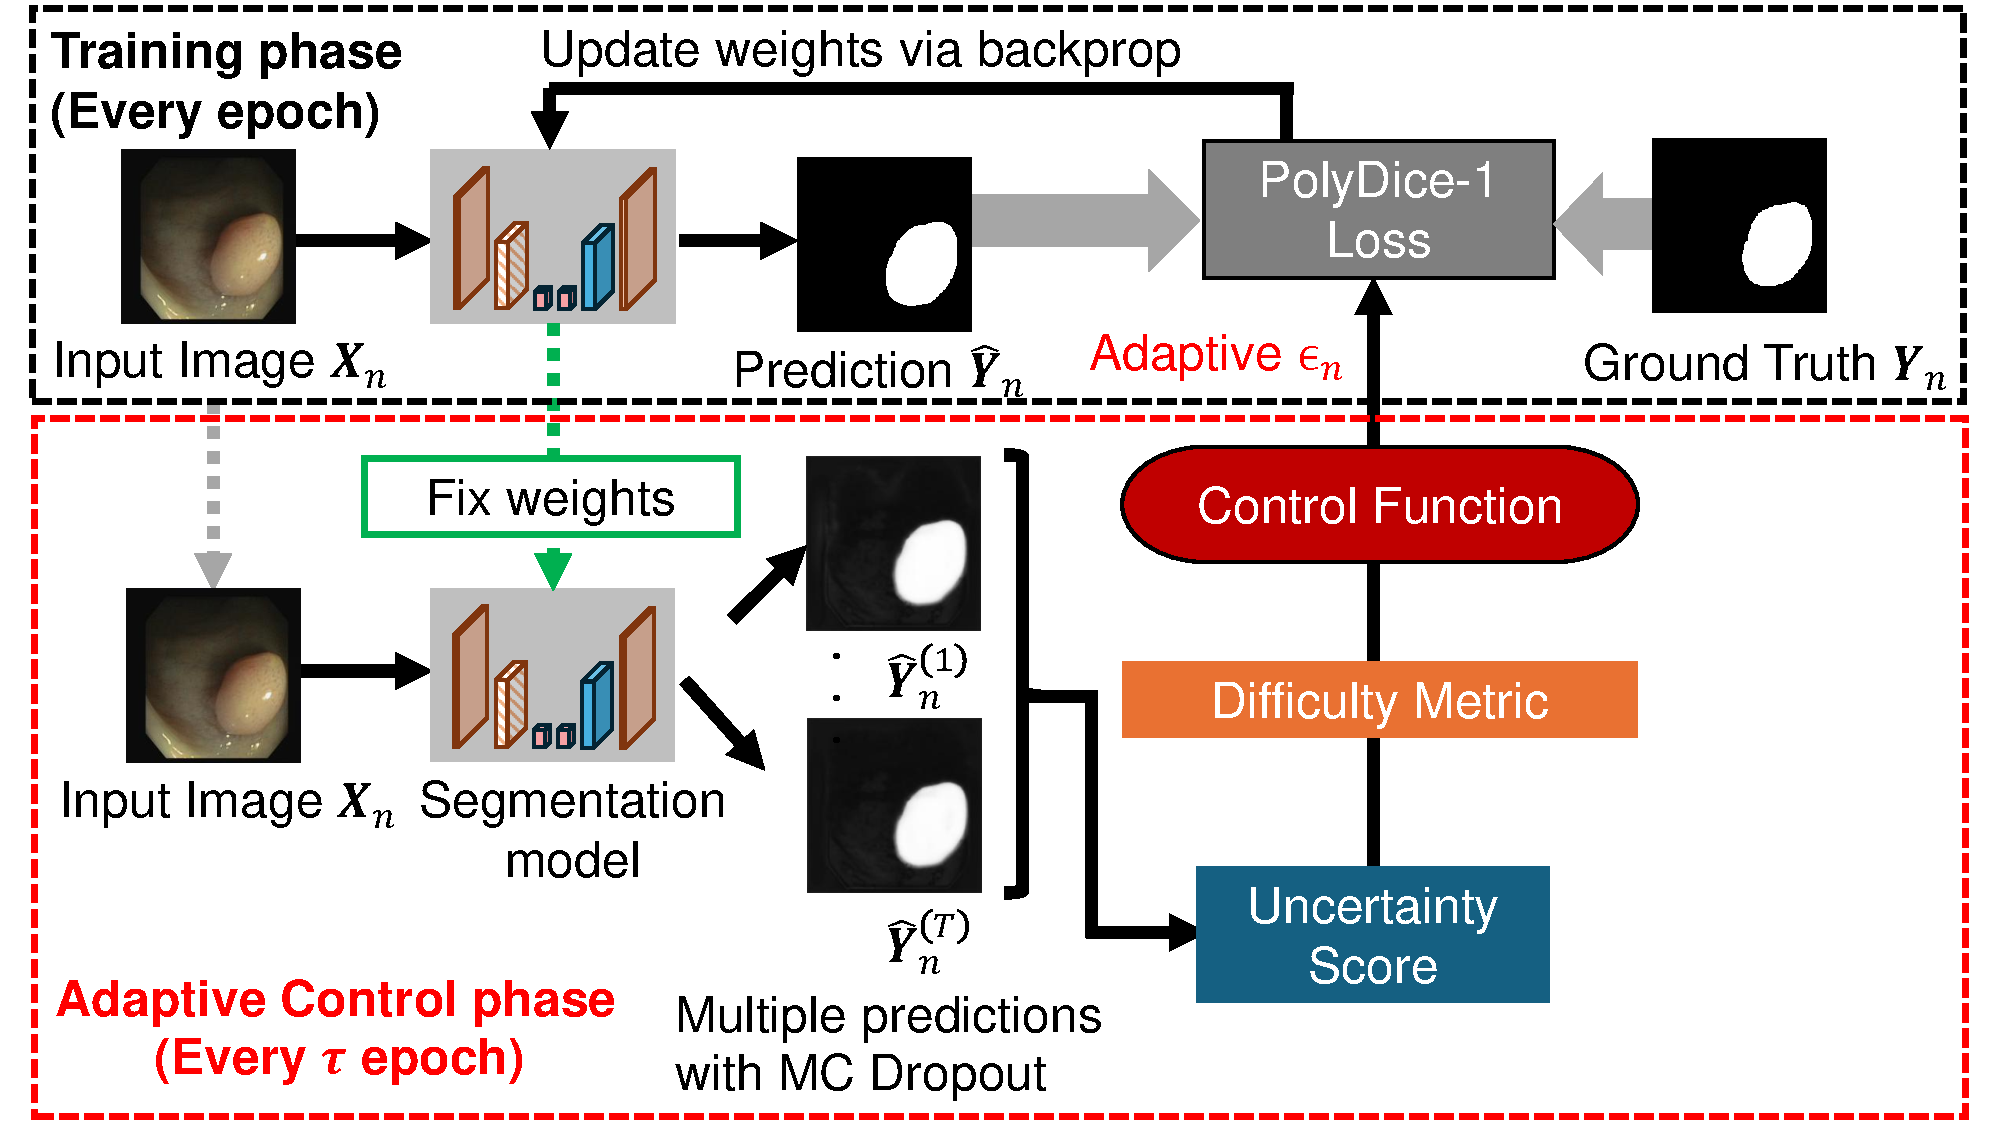
\includegraphics[width=\columnwidth]{figure/method.pdf}
    \caption{Overview of the proposed adaptive learning framework.
The process consists of two phases: uncertainty estimation and adaptive training. Every $\tau$ epochs, the model evaluates image difficulty using MC Dropout and updates the loss shape parameter $\epsilon$. This dynamic control assigns steeper gradients to harder samples, enabling difficulty-aware optimization.}
    \label{method}
\end{figure}

\subsection{不確実性に基づく画像難易度の定量化}

\subsubsection{学習中のMC Dropout推論}

提案法では，学習プロセスを初期学習期間と適応的学習期間の2段階に分割する．
エポック $1$ から $E_0 - 1$ までの期間は初期学習期間とし，損失形状パラメータ $\epsilon$ を$0$に固定して学習を行う．
この期間を設ける理由は，学習初期のモデルは特徴表現が未成熟であり，この段階での不確実性は画像の本質的な難易度よりもモデルの初期化に依存するためである．
$E_0$はモデルが基礎的なセグメンテーション能力を獲得するのに十分なエポック数として設定する．

適応的学習期間（$e \geq E_0$）においては，周期 $\tau$ ごとに不確実性の再評価と $\epsilon$ の更新を行う．
すなわち，更新は $e \in \{E_0, E_0+\tau, E_0+2\tau, \ldots\}$ を満たすエポックの学習開始前に実行される．
更新の際は，その時点のモデルパラメータ $\mathbf{W}$ を固定し，訓練データの各画像 $\mathbf{X}_n \in \{\mathbf{X}_n\}_{n=1}^{N}$ に対して Dropout 率 $p \in (0,1)$ で $T$ 回の確率的推論を行う．
得られる予測集合を $\{\hat{\mathbf{Y}}^{(n)}\}_{n=1}^{T}$ とする：
%
\begin{equation}
    \hat{\mathbf{Y}}^{(n)} = f_{\mathbf{W}}(\mathbf{X}_n; \mathbf{z}^{(n)}), \quad \mathbf{z}^{(n)} \sim \text{Bernoulli}(1-p)
\end{equation}
%
ここで，$\mathbf{z}^{(n)}$ は $n$ 回目の推論における Dropout マスクであり，$\hat{\mathbf{Y}}^{(n)}$ はその予測確率マップである．
この確率的推論により得られる予測のばらつきから，モデルの認識的不確実性を定量化する．

\subsubsection{ピクセル単位の不確実性指標の計算}
MC Dropoutによって得られた $T$ 枚の予測画像に対し，ピクセル単位の不確実性指標として
認識的不確実性を直接捉えることができる相互情報量 $I_{n, i, j}$ を計算する．

\begin{equation}
    I_{n, i,j} = \underbrace{H\left( \frac{1}{T} \sum_{t=1}^{T} \hat{y}_{n, i,j}^{(t)} \right)}_{\text{Entropy of Mean}} - \underbrace{\frac{1}{T} \sum_{t=1}^{T} H\left( \hat{y}_{n, i,j}^{(t)} \right)}_{\text{Mean of Entropy}}
\end{equation}

ここで，$H(p)$ は2値分類におけるバイナリ・エントロピー関数であり，次式で定義される．

\begin{equation}
    H(p) = -p \log p - (1-p) \log (1-p)
\end{equation}

相互情報量はモデルの予測に付随する不確実性を評価し，その依拠する要因を分離する指標として広く用いられている．
$T$ 回の推論結果を平均化した後の予測分布に対する不確実性であり，データとモデルの両方に由来する不確実性を示す予測エントロピーから，
個々の推論における不確実性の平均であり，
データ固有のノイズや曖昧さに由来する偶然的不確実性を示す期待エントロピーを減ずることで，認識的不確実性を定量化できる．
値が高い領域はモデルが十分に学習できていないことを示唆する．

\subsubsection{画像単位への集約}
ピクセル単位の相互情報量から外れ値を除去した後の平均値を，画像全体の難易度指標として定量化する．
医用画像セグメンテーションでは，背景領域が画像の大部分を占める一方で，関心領域である病変部は極めて小さいクラス不均衡が存在する．
背景領域は一般に推論が容易であり，その不確実性は極めて低い値をとる傾向がある． そのため，画像全体で不確実性の平均を算出すると，
大量の背景画素による低い値が難易度指標全体を支配してしまい，本来捉えるべき病変部の局所的な難易度を適切に定量化できない可能性がある．\\
したがって，病変検出の難易度を鋭敏に反映させるため，本手法では正解画像における病変領域に限定して相互情報量の平均を算出する．
画像領域全体を $\Omega_n$，正解マスクにおける陽性領域の画素集合を $\mathcal{P}_n = \{(i,j) \in \Omega \mid y_{i,j} = 1\}$ とする．
ここで，算出される相互情報量には突発的なノイズや極端な外れ値が含まれる可能性があり，これらが難易度指標の定量化を不安定にさせる要因となる．
そのため，スコアの算出に先立ち，統計的な外れ値除去を行う．
具体的には，領域 $\mathcal{P}_n$ 内の相互情報量の平均を $\mu_{\mathcal{P}_n}$，標準偏差を $\sigma_{\mathcal{P}_n}$ とし，有効な画素集合 $\mathcal{P}_n'$ を以下のように定義する．
\begin{equation}
    \mathcal{P}_n' = (i,j) \in \left\{\mathcal{P}_n \mid \mu_{\mathcal{P}_n} - 2\sigma_{\mathcal{P}_n} \leq I_{n, i, j} \leq \mu_{\mathcal{P}_n} + 2\sigma_{\mathcal{P}_n} \right\}
\end{equation}
ここで，閾値として $2\sigma_{\mathcal{P}_n}$ を採用した根拠は，統計的な信頼区間の考え方に基づく．
相互情報量の分布が正規分布に近似できると仮定した場合，平均値を中心とした $\pm 2\sigma$ の範囲内には全データの約 $95\%$ が含まれる．
したがって，この範囲外のデータを棄却することで，統計的に特異な極端値（外れ値）を効果的に除去しつつ，病変部の主要な特徴を反映したロバストな難易度推定が可能となる．
この有効集合 $\mathcal{P}_n'$ を用いて，画像全体の難易度スコア $D_n$ は次式で算出される．
\begin{equation}
    D_n = \frac{1}{|\mathcal{P}_n'|} \sum_{(i,j) \in \mathcal{P}_n'} I_{n, i,j}
\end{equation}
ここで，$|\mathcal{P}_n'|$ は外れ値除去後の陽性領域の画素数を表す．
なお，陽性領域が存在しない画像については，$D_n = 0$ とする．

次に，各サンプルの相対的な難易度を決定するため，データセット全体の難易度スコア分布に基づいて正規化を行う．
ここでの目的は，画像毎の数値的なスケールの差異を吸収し，各画像が分布全体の中で相対的にどの程度難しいかを評価することである．
データセット全体のスコア集合$\{D_n\}_{n = 1} ^ N$に対し， $q$ パーセンタイル値を $D_q$，標準偏差を $\sigma_D$ とすると，正規化されたスコア $D_{\text{norm}_n}$ は次のように計算される．

\begin{equation}
    D_{\text{norm}_n} = \frac{D_n - D_{q}}{\sigma_D + \delta}
\end{equation}
ここで，$\delta$ は数値的安定性のための微小定数である．
$D_q$ による減算は，後述する制御関数への入力を合わせるための中心化をする役割を持つ．
分布の平均値ではなく$q$パーセンタイル値を用いることで，容易なサンプルが多数を占める分布においても，
外れ値の影響を受けずに難易度の基準点を柔軟に設定できる．
$\sigma_D$ による除算は尺度の統一であり，
制御関数の感度がデータセットごとの不確実性のスケールに依存しないように調整する役割を持つ．

\subsection{適応的損失形状制御}

\subsubsection{制御関数の設計}
得られた難易度指標 $D_{\text{norm}_n}$ に基づき，PolyDice-1 Loss の形状パラメータ $\epsilon$ を動的に更新する．
更新式には以下のシグモイドベースの制御関数を用いる．

\begin{equation}
    \epsilon = \epsilon_{\text{min}} + (\epsilon_{\text{max}} - \epsilon_{\text{min}}) \sigma(k \cdot D_{\text{norm}_n})
\end{equation}
ここで，$\sigma(x) = (1 + e^{-x})^{-1}$標準シグモイド関数，$k > 0$ はパラメータであり，$\epsilon_{\text{min}}, \epsilon_{\text{max}}$ は $\epsilon$ の変動範囲である．

本手法でシグモイド関数を採用する理由は，有界性と滑らかさにある．
ステップ関数のような急激な切り替えは学習の安定性を損なう恐れがあり，
線形関数ではパラメータ$\epsilon$が適切な範囲$[\epsilon_{\text{min}}, \epsilon_{\text{max}}]$ を逸脱する可能性がある．
シグモイド関数を用いることで，難易度が低い領域から高い領域への遷移を滑らかに行いつつ，出力値を常に所定の範囲内に厳密に制約することが可能となる．
パラメータ $k$ は関数の応答感度を制御し，図\ref{sigmoid} に示すようにその値が大きいほど難易度判定の境界が急峻になり，小さいほど滑らかな遷移となる．

この制御により，難しい画像（$D_{\text{norm}_n}$が大きい）に対しては，大きな$\epsilon$を割り当て，
損失関数の勾配を急峻にする．これは，同じ予測誤差に対して
より大きな損失値と勾配を与えることを意味し，結果として難しい画像からの学習信号が相対的に強化される．
一方，すでに十分に学習できている簡単な画像には小さな$\epsilon$を割り当て，過学習を防ぎつつ学習リソースを難しい画像に集中させる．
更新された $\epsilon$ は学習に適用され，これによりモデルは困難な画像の学習を重点的に行うことが可能となる．

\begin{figure}
    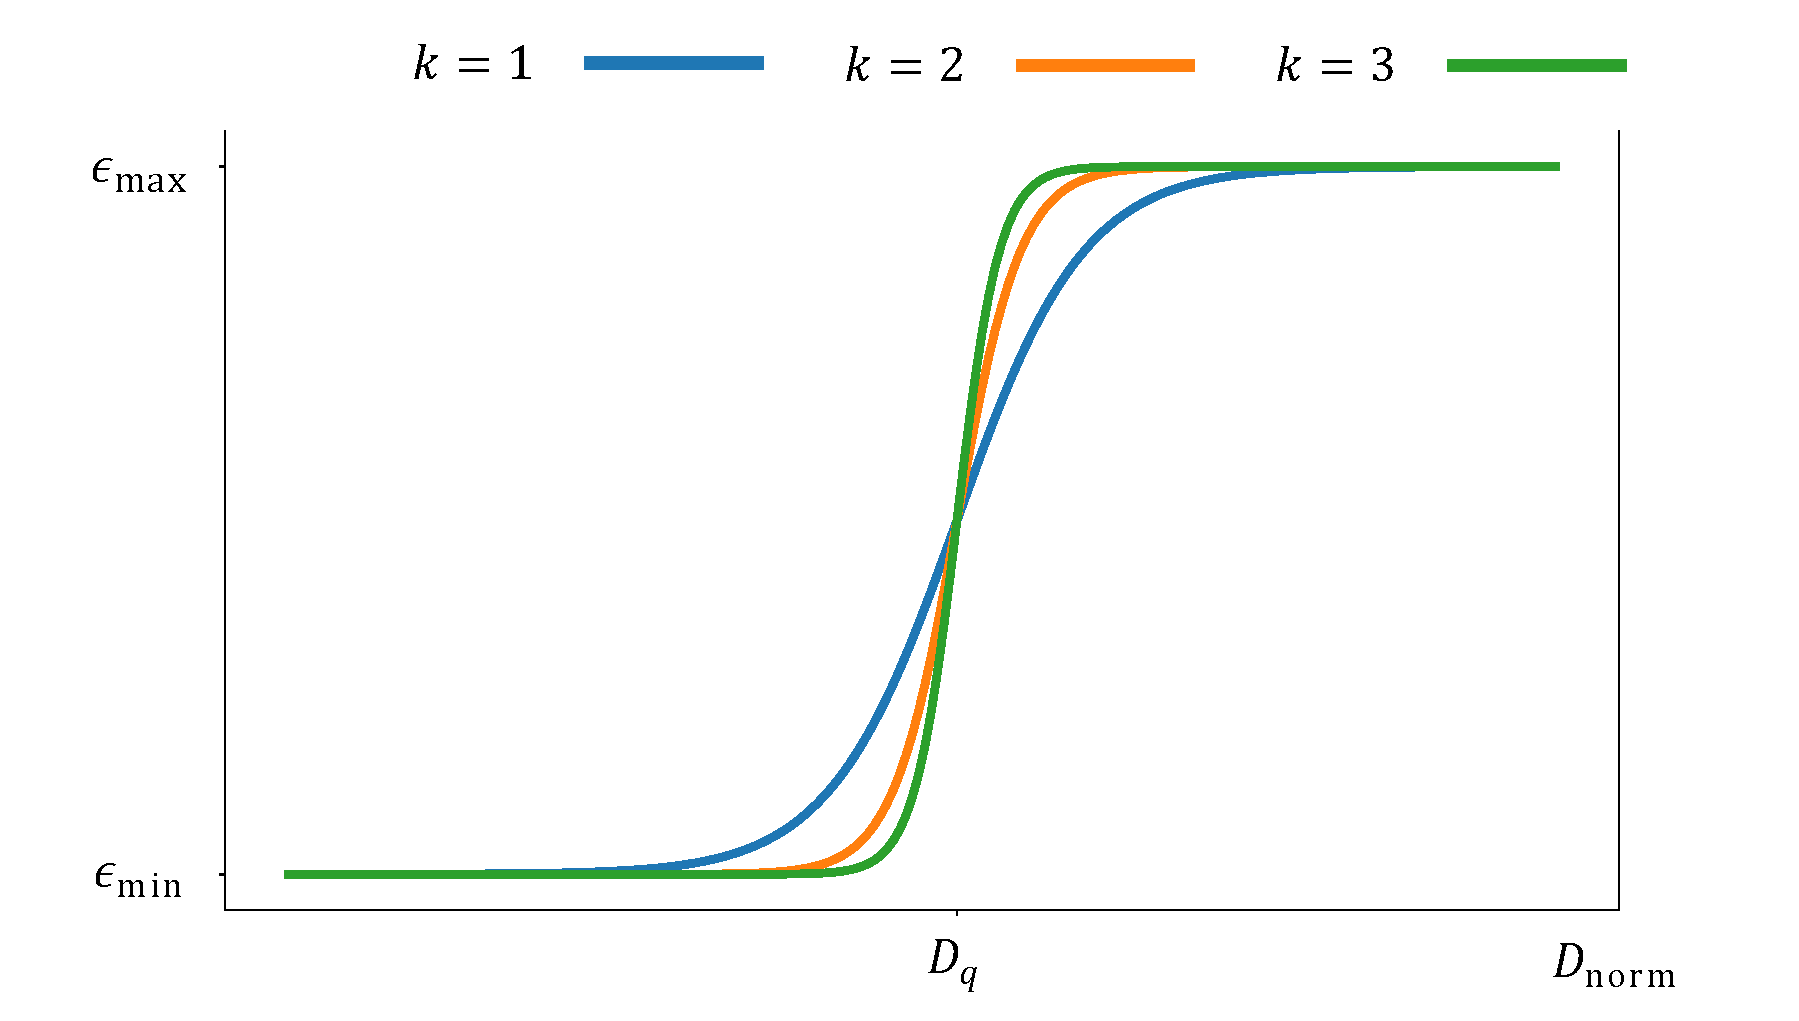
\includegraphics[width=\columnwidth]{figure/sigmoid_sensitivity.pdf}
    \caption{Sigmoid-based control function for loss shape parameter $\epsilon$}
    \label{sigmoid}
\end{figure}

\subsubsection{学習アルゴリズム}
アルゴリズム\ref{alg:proposed_method} に詳細なアルゴリズムを示す．
学習プロセスは難易度評価と損失パラメータ更新を行う適応的制御と，
実際にモデルパラメータを更新する学習段階の2つで構成される．

学習開始時，モデルパラメータ $\mathbf{W}$ を初期化し，全ての画像に対する損失形状パラメータ $\epsilon$ を $0$ に初期化する．
$E_0 > 0$の場合，エポック $1$ から $E_0 - 1$までの期間は初期学習期間とし，
$\epsilon=0$を固定して標準的なPolyDice-1 Lossで学習を行う．この期間により，モデルは不確実性推定に必要な基礎的な特徴表現を獲得する．
$E_0 = 0$の場合は，最初のエポックから適応的制御を開始する．

適応的学習期間（$e \geq E_0$）では，$\tau$ エポックごとに適応的制御が実行される．
ここでは，3.2節で述べた手順に従い，MC Dropout推論による不確実性指標推定，画像単位への集約，正規化を経て，各画像の $\epsilon$ が更新される．
適応的制御の段階ではモデルパラメータ$\mathbf{W}$は固定されており，損失関数の形状パラメータ$\epsilon$の更新のみが行われることに注意されたい．

続く学習段階（Epoch $e$）では，更新された $\epsilon$ を用いてミニバッチ学習を行う．
具体的には，ランダムにサンプリングされたミニバッチを構成する画像のインデックス集合を $\mathcal{B} \subset \{1, \dots, N\}$ とする．
このとき，最適化の対象となる目的関数 $\mathcal{L}$ は，バッチ内の各画像 $n \in \mathcal{B}$ に個別に割り当てられた形状パラメータ $\epsilon_n$ を用いた PolyDice-1 Loss の平均として次式で定義される．

\begin{equation}
    \mathcal{L} = \frac{1}{|\mathcal{B}|} \sum_{n \in \mathcal{B}} \mathcal{L}_{\text{PolyDice-1}}(\hat{\mathbf{Y}}_n, \mathbf{Y}_n; \epsilon_n)
\end{equation}

ここで，$\mathcal{L}_{\text{PolyDice-1}}(\cdot; \epsilon_n)$ はパラメータ $\epsilon_n$ を適用した単一画像の損失関数を表す．
このように，バッチ内の各画像に対して異なる $\epsilon_n$ を適用することで，
難易度が高いと判定された画像には急峻な勾配を，低い画像には緩やかな勾配を同時に与えることが可能となる．
最終的に，この損失関数 $\mathcal{L}$ に基づく勾配降下法により，モデルパラメータ $\mathbf{W}$ が最適化される．
このサイクルを繰り返すことで，モデルの学習に応じて困難な画像の学習を重点的に行うことが可能となる．

\begin{algorithm}[t]
    \caption{Uncertainty-based Adaptive PolyDice-1 Loss Learning Algorithm}
    \label{alg:proposed_method}
    \begin{algorithmic}[1]
        \small
        \Require Training dataset $\mathcal{D} = \{(\mathbf{X}_n, \mathbf{Y}_n)\}_{n=1}^{N}$
        \Require Model $f_{\mathbf{W}}$, Max epochs $E$
        \Require \textbf{Hyperparameters:} Dropout probability $p$, Start epoch $E_0$, Interval $\tau$, MC iterations $T$, Normalization percentile $q$, Slope $k$, Range $[\epsilon_{\text{min}}, \epsilon_{\text{max}}]$
        
        \State Initialize model parameters $\mathbf{W}$
        \State Initialize loss parameters $\epsilon_n \leftarrow 0$ for all $n \in \{1, \dots, N\}$
        
        \For{$e = 1$ \textbf{to} $E$}
            \If{$e \geq E_0$ \textbf{and} $(e - E_0) \pmod \tau = 0$}
                \State Set model to evaluation mode (enable Dropout)
                
                \For{$n = 1$ \textbf{to} $N$}
                    \For{$t = 1$ \textbf{to} $T$}
                        \State $\hat{\mathbf{Y}}^{(t)} = f_{\mathbf{W}}(\mathbf{X}_n; \mathbf{z}^{(t)}), \quad \mathbf{z}^{(t)} \sim \text{Bernoulli}(1-p)$
                    \EndFor
                    
                    \State Calculate pixel-wise Mutual Information (Eq. 9):
                    \State $I_{n, i,j} = H\left( \frac{1}{T} \sum_{t=1}^{T} \hat{y}_{n, i,j}^{(t)} \right) - \frac{1}{T} \sum_{t=1}^{T} H\left( \hat{y}_{n, i,j}^{(t)} \right)$
                    
                    \If{positive region $\mathcal{P}_n \neq \emptyset$}
                        \State Compute $\mu_{\mathcal{P}_n}, \sigma_{\mathcal{P}_n}$ from $\{I_{n,i,j} \mid (i,j) \in \mathcal{P}_n\}$
                        \State Identify valid pixels: $\mathcal{P}_n' = \{(i,j) \in \mathcal{P}_n \mid |I_{n,i,j} - \mu_{\mathcal{P}_n}| \leq 2\sigma_{\mathcal{P}_n} \}$
                        \State $D_n = \frac{1}{|\mathcal{P}_n'|} \sum_{(i,j) \in \mathcal{P}_n'} I_{n, i,j}$
                    \Else
                        \State $D_n \leftarrow 0$ \Comment{Handle negative samples}
                    \EndIf
                \EndFor

                \State \textbf{Step 2: Normalization \& $\epsilon$ Update}
                \State Compute $q$-percentile $D_q$ and std $\sigma_D$ from $\{D_n\}_{n=1}^N$
                \For{$n = 1$ \textbf{to} $N$}
                    \State Normalize score (Eq. 13): $D_{n, \text{norm}} = \frac{D_n - D_{q}}{\sigma_D + \delta}$
                    \State Update $\epsilon_n$ (Eq. 14): $\epsilon_n \leftarrow \epsilon_{\text{min}} + (\epsilon_{\text{max}} - \epsilon_{\text{min}}) \sigma(k \cdot D_{n, \text{norm}})$
                \EndFor
            \Else
                \State \Comment{Keep current $\epsilon_n$ (Note: $\epsilon_n=0$ if $e < E_0$)}
            \EndIf

            \State
            \State Set model to training mode (disable MC Dropout)
            \For{each minibatch $\mathcal{B} \subset \{1, \dots, N\}$}
                \State Compute batch loss with sample-specific $\epsilon_n$ (Eq. 15):
                \State \quad $\mathcal{L} = \frac{1}{|\mathcal{B}|} \sum_{n \in \mathcal{B}} \mathcal{L}_{\text{PolyDice-1}}(\hat{\mathbf{Y}}_n, \mathbf{Y}_n; \epsilon_n)$
                \State Update parameters: $\mathbf{W} \leftarrow \mathbf{W} - \eta \nabla_{\mathbf{W}} \mathcal{L}$
            \EndFor
        \EndFor
        \State \Return Trained parameters $\mathbf{W}$
    \end{algorithmic}
\end{algorithm}

\section{実験}
\subsection{実験設定}
\subsubsection{データセット}
CVC-ClinicDBデータセット\cite{BERNAL201599}データセットおよびKvasir-SEGデータセット\cite{jha2020kvasir}を用いて実験を行った．
CVC-ClinicDBデータセットは$612$枚の大腸内視鏡画像（$384 \times 288$ pixel），Kvasir-SEGデータセットは$1000$枚の大腸内視鏡画像で，
いずれも大腸内視鏡画像とそれに対応するポリープの正解マスクから構成される．
データは$5$分割交差検証で分割され，CVC-ClinicDBデータセットに関しては同一のビデオシーケンスが異なるfoldに跨がらないよう，GroupKFoldを用いた分割を行った．

\subsubsection{実装の詳細}
セグメンテーションモデルには表\ref{tab:unet_architecture}に示される構造のU-Net\cite{ronneberger2015u}を採用した．
学習にはAdam optimizer\cite{kingma2014adam}を使用し，バッチサイズ$32$, 学習率$10 ^ {-3}$に設定した．
前処理として全画像を$W = 224$ pixel, $H = 224$ pixelにリサイズし，訓練時には
$50\%$の確率で上下左右反転および明度・コントラストの変更を適用した．
最大エポック数$E$は$200$に設定した．

MC Dropoutによる不確実評価は，$\tau=10$エポックごとに実施した．
Dropout層はエンコーダの最終ブロックとデコーダの最終ブロックに配置し，
各評価時には，先行研究\cite{pmlr-v48-gal16}を基に$p = 0.5$で$T = 10$回の確率的推論を行った．
またデータセット内の難易度指標の正規化時のパーセンタイルは難易度分布の偏りを考慮して$q = 25$に設定し，
予備実験の結果を基に適応的学習の開始エポックは$E_0 = 10$とし，
$\epsilon_{\text{min}}=0$, $\epsilon_{\text{max}}=0.5$, $k=2$とした．


\subsubsection{比較条件}
適応的学習の有効性を評価するため，以下の手法と提案法を比較する：

\begin{itemize}
    \item Dice Loss\cite{milletari2016v}：医用画像セグメンテーションにおける標準的な損失関数であり，ベースラインとして採用した．
    \item Focal Loss\cite{lin2017focal}：易しいサンプルの損失を down-weight することで
    クラス不均衡に対処する手法であり，
    提案法と「サンプルの難易度に応じた重み付け」という点で動機が共通する．
    ただし，Focal Loss は予測確信度に基づく静的な重み付けであるのに対し，
    提案法はモデルの不確実性に基づく動的な重み付けである点が異なる．
    また易しいサンプルの損失を down-weight する割合は$\gamma = 2$とした．
    \item PolyDice-1 Loss ($\epsilon = 0$)：PolyDice-1 Loss の標準形式であり，
    理論上は通常の Dice Lossを近似したものである．
    提案法および後述する Optimal 設定との比較において，
    パラメータ $\epsilon$ を操作すること自体の純粋な効果を検証するための基準として採用した．
    \item PolyDice-1 Loss (optimal)：固定$\epsilon$による性能の理論的上界を評価するため，
    テストデータに対する Dice 係数を最大化する$\epsilon$値を事後的に探索し，
    これを理想設定として比較に含めた．具体的には，
    $\epsilon \in \{-0.3, -0.2, \ldots, 0.5\}$ の範囲で網羅的に評価し，
    最高精度を達成する値$\epsilon$をデータセットごとに決定した．
    この設定は実運用では実現不可能であるが，
    「最適な固定値が事前に既知である」という理想的な条件下での性能を表す．
\end{itemize}

これらの比較により，(1) 提案法が標準的な損失関数より優れているか，
(2) 適応的$\epsilon$制御が固定$\epsilon = 0$より有効か，(3) 提案法が Optimal 設定に匹敵あるいは上回る性能を達成できるか，を検証する．

\subsubsection{評価指標}

またセグメンテーションの性能の評価には，領域の重なりを測るDice係数およびIoUおよび検出精度を測るPrecisionおよびRecallを用いた．
モデルの予測マップ $\hat{Y}_n$に対し，閾値 $\theta_\text{th} = 0.5$ で二値化した予測マスク $\tilde{Y}_n = \{\tilde{y}_{n,i,j}\}$ とする．
画像$n$に対する真陽性 (TP)，偽陽性 (FP)，偽陰性 (FN) の画素数はそれぞれ以下で定義される．

\begin{align}
    TP_n &= \sum_{j=1}^{W} \sum_{i=1}^{H} \tilde{y}_{i, j} y_{i, j} \\
    FP_n &= \sum_{j=1}^{W} \sum_{i=1}^{H} \tilde{y}_{i, j} (1 - y_{i, j}) \\
    FN_n &= \sum_{j=1}^{W} \sum_{i=1}^{H} (1 - \tilde{y}_{i, j}) y_{i, j}
\end{align}

\begin{itemize}
    \item Dice係数: 正解領域と予測領域の重複度を直接評価するもので，医用画像のような不均衡な画像でも，微小な対象物の抽出精度を適切に反映できるため，主指標として採用した．
    \begin{align}
        \text{Dice}_n = \frac{2TP_n}{2TP_n + FP_n + FN_n}
        % &= \frac{2TP}{2TP + FP + FN}
    \end{align}

    \item IoU：予測領域と正解領域の共通部分を評価する指標であり，セグメンテーションタスクにおける一般的な評価指標として広く用いられている．
    \begin{align}
        \text{IoU}_n = \frac{TP_n}{TP_n + FP_n + FN_n}
    \end{align}

    \item Precision：モデルが抽出した領域の正解率を評価する指標であり，過剰な検出を抑制する性能を定量化するために採用した．
    \begin{align}
        \text{Precision}_n = \frac{TP_n}{TP_n + FP_n}
    \end{align}

    \item Recall：正解領域をどの程度検出できているかを評価する指標であり，特に病変の見落としを防ぐ性能を検証するために採用した．
    \begin{align}
        \text{Recall}_n = \frac{TP_n}{TP_n + FN_n}
    \end{align}
\end{itemize}

各指標はテストデータ全体での平均値を報告する．

\clearpage

\begin{table}[t]
    \centering
    \caption{Overview of the U-Net Architecture}
    \label{tab:unet_architecture}
    \begin{tabular}{lc}
        \toprule
        \textbf{Layer} & \textbf{Output Size} \\
        \midrule
        % ★★★ 表示するテキストを追加 ★★★
        \multicolumn{2}{c}{\textit{--- Encoder ---}} \\
        Input & $224 \times 224 \times 3$ \\
        inc (DoubleConv) & $224 \times 224 \times 64$\\
        down1 (MaxPool + DoubleConv) & $112 \times 112 \times 128$ \\
        down2 (MaxPool + DoubleConv) & $56 \times 56 \times 256$ \\
        down3 (MaxPool + DoubleConv) & $28 \times 28 \times 512$ \\
        down4 (MaxPool + DoubleConv) & $14 \times 14 \times 512$ \\
        \midrule
        % ★★★ 表示するテキストを追加 ★★★
        \multicolumn{2}{c}{\textit{--- Decoder ---}} \\
        up1 (Upsample + DoubleConv) & $28 \times 28 \times 256$ \\
        up2 (Upsample + DoubleConv) & $56 \times 56 \times 128$ \\
        up3 (Upsample + DoubleConv) & $112 \times 112 \times 64$ \\
        up4 (Upsample + DoubleConv) & $224 \times 224 \times 64$ \\
        \midrule
        outc (Conv2d) & $224 \times 224 \times 2$ \\
        \bottomrule
    \end{tabular}
\end{table}

\clearpage

\begin{table}[t]
    \centering
    \caption{Performance Comparison with Existing Loss Functions on CVC-ClinicDB Dataset}
    \label{tab:benchmark_cvc_clinicdb}
    \begin{tabular}{ccccc} % lcccc から ccccc に変更（全て中央揃え）
        \toprule
        Method & Dice & IoU & Precision & Recall \\ % Dice Coefficient -> Dice に短縮
        \midrule
        Dice Loss & 0.5408 & 0.4347 & 0.6359 & 0.5819 \\
        Focal Loss ($\gamma = 2$) & 0.5007 & 0.4133 & 0.7078 & 0.4707 \\
        PolyDice-1 ($\epsilon=0$) & 0.5825 & 0.4808 & 0.6817 & 0.6167 \\ % fixed, .0 を削除
        PolyDice-1 (Opt. $\epsilon$) & 0.6145 & 0.5145 & 0.7090 & 0.6372 \\ % optimized, fixed を短縮
        \midrule
        Adaptive PolyDice-1 & \textbf{0.6924} & \textbf{0.5262} & \textbf{0.7827} & \textbf{0.7113} \\
    \bottomrule
    \end{tabular}
\end{table}

\begin{table}[t]
    \centering
    \caption{Performance Comparison with Existing Loss Functions on Kvasir-SEG Dataset}
    \label{tab:benchmark_kvasir_seg}
    \begin{tabular}{ccccc} % lcccc から ccccc に変更（全て中央揃え）
        \toprule
        Method & Dice & IoU & Precision & Recall \\ % Dice Coefficient -> Dice に短縮
        \midrule
        Dice Loss & 0.7895 & 0.7021 & 0.8281 & 0.8154 \\
        Focal Loss ($\gamma = 2$) & 0.7192 & 0.6082 & 0.8634 & 0.6769 \\
        PolyDice-1 ($\epsilon=0$) & 0.8095 & 0.7198 & 0.8461 & 0.8268 \\ % fixed, .0 を削除
        PolyDice-1 (Opt. $\epsilon$) & 0.8095 & 0.7198 & 0.8461 & 0.8268 \\ % optimized, fixed を短縮
        \midrule
        Adaptive PolyDice-1 & \textbf{0.8272} & \textbf{0.7440} & \textbf{0.8707} & \textbf{0.8397} \\
    \bottomrule
    \end{tabular}
\end{table}

\begin{table}[t]
    \centering
    \caption{Performance evaluation of PolyDice-1 Loss with fixed $\epsilon$ on CVC-ClinicDB Dataset}
    % \caption{Performance Comparison with Existing Loss Functions on Kvasir-SEG Dataset}
    \label{tab:polydice_fixed_epsilon_cvc}
    \begin{tabular}{ccccc} % lcccc から ccccc に変更（全て中央揃え）
        \toprule
        Coefficient & Dice & IoU & Precision & Recall \\ % Dice Coefficient -> Dice に短縮
        \midrule
        -0.3 & 0.5713 & 0.4705 & 0.6641 & 0.6190 \\
        -0.2 & 0.6102 & 0.5089 & 0.6991 & 0.6515 \\
        -0.1 & 0.6007 & 0.5010 & 0.6972 & 0.6302 \\ % fixed, .0 を削除
        0.0 & 0.5825 & 0.4808 & 0.6817 & 0.6167 \\ % optimized, fixed を短縮
        0.1 & 0.5823 & 0.4876 & 0.7056 & 0.5893 \\
        0.2 & 0.6145 & 0.5145 & 0.7090 & 0.6372 \\
        0.3 & 0.5933 & 0.4947 & 0.6990 & 0.6035 \\
        0.4 & 0.6047 & 0.5052 & 0.7002 & 0.6198 \\
        0.5 & 0.5757 & 0.4748 & 0.7062 & 0.5958 \\
    \bottomrule
    \end{tabular}
\end{table}

\begin{table}[t]
    \centering
    \caption{Performance evaluation of PolyDice-1 Loss with fixed $\epsilon$ on Kvasir-SEG Dataset}
    % \caption{Performance Comparison with Existing Loss Functions on Kvasir-SEG Dataset}
    \label{tab:polydice_fixed_epsilon_kvasir-seg}
    \begin{tabular}{ccccc} % lcccc から ccccc に変更（全て中央揃え）
        \toprule
        Coefficient & Dice & IoU & Precision & Recall \\ % Dice Coefficient -> Dice に短縮
        \midrule
        -0.3 & 0.8036 & 0.7174 & 0.8435 & 0.8219 \\
        -0.2 & 0.7284 & 0.6266 & 0.7934 & 0.7558 \\
        -0.1 & 0.7357 & 0.6351 & 0.7918 & 0.7658 \\ % fixed, .0 を削除
        0.0 & 0.8095 & 0.7198 & 0.8461 & 0.8268 \\ % optimized, fixed を短縮
        0.1 & 0.7971 & 0.7111 & 0.8375 & 0.8174 \\
        0.2 & 0.7964 & 0.7077 & 0.8268 & 0.8231 \\
        0.3 & 0.7966 & 0.7083 & 0.8301 & 0.8243 \\
        0.4 & 0.8024 & 0.7157 & 0.8305 & 0.8346 \\
        0.5 & 0.7356 & 0.6358 & 0.7910 & 0.7635 \\
    \bottomrule
    \end{tabular}
\end{table}

\clearpage

\subsection{結果と議論}

\subsubsection{比較手法との性能比較：}
全データセットでの比較表

\subsubsection{難易度別の性能分析}
群ごとの性能比較，εの推移や分布の推移

\subsubsection{不確実性指標の妥当性検証}
予測平均と相互情報量の推移を示す

\subsubsection{ハイパーパラメータの影響}
\begin{enumerate}
    \item ε範囲の影響
    \begin{enumerate}
        \item $\epsilon \in [0, 0.3]$ (控えめ)
        \item $\epsilon \in [0, 0.5]$ (標準)
        \item $\epsilon \in [-0.3, 0.5]$ (双方向)
    \end{enumerate}

    \item 適応速度$k$の影響
    \begin{enumerate}
        \item $k=1$
        \item $k=2$
        \item $k=3$
    \end{enumerate}

    \item 適応開始タイミング$E_0$の影響
    \begin{enumerate}
        \item $E_0=10$
        \item $E_0=60$
        \item $E_0=110$
        \item $E_0=160$
    \end{enumerate}
\end{enumerate}

% \begin{table}[t]
%     \centering
%     \caption{Impact of Different $\epsilon$ Ranges on Segmentation Performance CVC-ClinicDB Dataset}
%     \label{tab:ablation_epsilon_cvc}
%     \begin{tabular}{ccccc}
%         \toprule
%         $\epsilon_{\text{min}}$ & $\epsilon_{\text{max}}$ & Dice & IoU & Precision & Recall \\
%         \midrule
%         $0$ & $0.3$ & 0.6935 & 0.5962 & 0.7853 & 0.7175 \\
%         $0$ & $0.5$ & 0.6924 & 0.5913 & 0.7827 & 0.7113 \\
%         $-0.3$ & $0.5$ & 0.8189 & 0.7313 & 0.8537 & 0.8454 \\
%         \bottomrule
%     \end{tabular}
% \end{table}

\begin{table}[t]
    \centering
    \caption{Impact of Different $\epsilon$ Ranges on Segmentation Performance Kvasir-SEG Dataset}
    \label{tab:ablation_epsilon_kvasir-seg}
    \begin{tabular}{cccccc}
        \toprule
        $\epsilon_{\text{min}}$ & $\epsilon_{\text{max}}$ & Dice & IoU & Precision & Recall \\
        \midrule
        $0$ & $0.3$ & 0.8239 & 0.7391 & 0.8608 & 0.8410 \\
        $0$ & $0.5$ & 0.8272 & 0.7440 & 0.8707 & 0.8397 \\
        $-0.3$ & $0.5$ & 0.8189 & 0.7313 & 0.8537 & 0.8454 \\
        \bottomrule
    \end{tabular}
\end{table}

% \begin{table}[t]
%     \centering
%     \caption{Performance Sensitivity to Slope Parameter $k$ CVC-ClinicDB Dataset}
%     \label{tab:ablation_k_cvc}
%     \begin{tabular}{ccccc}
%         \toprule
%         Slope ($k$) & Dice & IoU & Precision & Recall \\
%         \midrule
%         $1$ & 0.6935 & 0.5962 & 0.7853 & 0.7175 \\
%         $2$ & 0.6924 & 0.5913 & 0.7827 & 0.7113 \\
%         $3$ & 0.0000 & 0.0000 & 0.0000 & 0.0000 \\
%         \bottomrule
%     \end{tabular}
% \end{table}

\begin{table}[t]
    \centering
    \caption{Performance Sensitivity to Slope Parameter $k$ Kvasir-SEG Dataset}
    \label{tab:ablation_k_kvasir-seg}
    \begin{tabular}{ccccc}
        \toprule
        $k$ & Dice & IoU & Precision & Recall \\
        \midrule
        $1$ & 0.8235 & 0.7404 & 0.8589 & 0.8440 \\
        $2$ & 0.8272 & 0.7440 & 0.8707 & 0.8397 \\
        $3$ & 0.8229 & 0.7375 & 0.8663 & 0.8370 \\
        \bottomrule
    \end{tabular}
\end{table}

% \begin{table}[t]
%     \centering
%     \caption{Effect of Adaptation Start Epoch $E_0$ CVC-ClinicDB Dataset}
%     \label{tab:ablation_e0_cvc}
%     \begin{tabular}{ccccc}
%         \toprule
%         $E_0$ & Dice & IoU & Precision & Recall \\
%         \midrule
%         $10$ & 0.6924 & 0.5962 & 0.7827 & 0.7113 \\
%         $60$ & 0.8097 & 0.7226 & 0.8571 & 0.8255 \\
%         $110$ & 0.6325 & 0.5262 & 0.7328 & 0.6522 \\
%         $160$ & 0.5940 & 0.4920 & 0.7138 & 0.6123 \\
%         \bottomrule
%     \end{tabular}
% \end{table}

\begin{table}[t]
    \centering
    \caption{Effect of Adaptation Start Epoch $E_0$ Kvasir-SEG Dataset}
    \label{tab:ablation_e0_kvasir-seg}
    \begin{tabular}{ccccc}
        \toprule
        $E_0$ & Dice & IoU & Precision & Recall \\
        \midrule
        $10$ & 0.8272 & 0.7440 & 0.8707 & 0.8397 \\
        $60$ & 0.8097 & 0.7226 & 0.8571 & 0.8255 \\
        $110$ & 0.8136 & 0.7250 & 0.8574 & 0.8309 \\
        $160$ & 0.8005 & 0.7125 & 0.8480 & 0.815 \\
        \bottomrule
    \end{tabular}
\end{table}

\subsubsection{定性的評価}
失敗例の分析，提案法でも失敗する症例の特徴分析，今後の改善方向を示唆

\section{文献引用}
文献引用の例を次に示します．
\newline

レンダリング方程式（rendering equation）~\cite{kajiya1986rendering}は，算出すべき放射輝度$L$が式の両辺に表れた積分方程式となっている．

フォトンマッピング法~\cite{jensen2001realistic}では2段階のレイトレーシングを行うことによりレンダリング方程式を解く．


\section{まとめ}
卒業論文発表予稿の様式を示しました．


\bibliographystyle{bibstyle}
\bibliography{bib}

\end{document}